\chapter{\textsc{Literature Survey}}
\label{chapter:literature_survey}

During the process of making a proposal, one of the tasks that researchers complete is the classification of the project using one or more research topics. By doing this, researchers use their judgement and provide intelligence in regards to the similarity between two grants based on topics and also the relationship between two topics based on grants. 

A problem concerning the way topics within EPSRC are defined exists. It is not known how finely or coarsely the topics should be defined and how to define them in either way. This problem may arise when there are too many similar topics or not enough topics to cover the full topic classification spectrum of the grants. The relatedness of topics is also unknown. Currently, there are no known solutions or attempts to address the problem.

This project aims to identify a solution to the problem by using a novel approach involving graph theory and the concept of modularity. Focusing on grants that are classified by two or more topics, a network of topics can be constructed with the links between topics representing one or more common grants. Initially, within the network of topics constructed, there is no distinction between topics, apart from their names and links to other topics. Attempting to determine how topics should be defined while at the same time, focusing on the full network will prove extremely difficult. Subsequently, grouping similar topics manually, and analysing each group separately would lower the difficulty level, but will significantly increase the time it would take to complete the task.

In the end, the problem becomes a clustering problem, a very specific one, concerned with identifying the optimal way of dividing the network into clusters of topics in a rational and efficient manner. Furthermore, there are many other clustering problems in other fields such as \textit{document clustering} which share some common ground with the problem addressed in this project. Furthermore, other fields are related to the approach used in this project including \textit{topic modelling} and \textit{document classification}.

This chapter presents the latest development in a number of related topics, while it also introduces the state-of-the-art in \textit{network analysis}, the main topic of this project.

\section{Topic modelling}

\textit{Topic Modelling} represents a type of statistical model used to discover hidden topical structures within the text body of a document which is part of a document collection. It has become extremely popular over the years, with 17,043 research papers on Topic Modelling published since 2015, according to the ACM Digital Library \cite{acm_digital_library}.

In 2016, Gong et al. published \textit{Who Will You @?} \cite{gong2015will} which involves the development of a recommendation system focused on the mention function in microblogging services. In the process of recommendation, they system takes into consideration both the content of the microblog and the histories of candidate users. Moreover, a novel method which extends the translation-based model is proposed as a better way to handle the textual information. Experiments are carried out using a real-world data set collected from microblogging services. The results of the experiments prove that the proposed solution performed better than the previous state-of-the-art approaches.

In recent years, social media has cemented its popularity in the field of \textit{topic modelling} as more and more researchers are attracted by the opportunity to analyse large volumes of text which are provided in data sets collected from social media services such as Facebook or Twitter.

This observation is justified by Sokolova et al. who, also in 2016, published \textit{Topic Modelling and Event Identification from Twitter Textual Data} \cite{sokolova2016topic}, which focuses on the analysis of four data sets of Twitter messages regarding challenging social events in Kenya. The \textit{Latent Dirichlet Allocation (LDA)} model is used to analyse the text content, while the study is evaluated using both \textit{Normalized Mutual Information (NMI)} and \textit{topic coherence analysis}, in order to identify the optimal LDA models. This study concludes that the tool developed has an effective use in the extraction of discussion topics for further manual analysis.

\section{Document clustering}

\textit{Document clustering} is the process of applying clustering analysis to textual documents. Its use is divided between different fields such as topic extraction, fast information retrieval and document organisation. In contrast to \textit{topic modelling}, the field of \textit{document clustering} is not as popular, with 4,069 research papers listed in the ACM Digital Library \cite{acm_digital_library}, since 2015.

\textit{World Knowledge as Indirect Supervision for Document Clustering} \cite{wang2016world} was published by Wang et al. in 2016, and proposes a solution to the key obstacle that arises in making learning protocols realistic in applications, which is the need for supervision. Supervision represents a costly process as the involvement of domain experts is often required. The solution proposed represents a framework using world knowledge as indirect supervision. Furthermore, an example of using world knowledge for domain dependent document clustering is presented. Extensive experiments are carried out on several text benchmark data sets including \textit{20newsgroups} and \textit{Freebase}. The results of the experiments showed that incorporating world knowledge as indirect supervision is capable to outperform the state-of-the-art clustering algorithms as well as the ones enhanced with world knowledge features.

In contrast to the social-media focus identified in the latest \textit{topic modelling} research, the research in the \textit{document clustering} domain is much more varied. In 2016, Tripodi and Pellilo focused on \textit{Document Clustering Games in Static and Dynamic Scenarios} \cite{tripodi2016document}, which proposes a game theoretic model for document clustering. In the game, each document to be clustered is a player and each cluster is a strategy. By interacting with others, players receive rewards. The game model is evaluated using 13 document collections using several different experiment settings. Compared to other document clustering algorithms, the results prove that the proposed solution performs well.

\section{Document classification}

In contrast to \textit{document clustering}, \textit{document classification} represents a problem in computer, information and library science that deals with the categorisation of a document into one or more categories.

However, similarities between the \textit{document clustering} and \textit{document classification} fields also exist in terms of popularity and research trend. Since 2015, according to the ACM Digital Library \cite{acm_digital_library}, 3,941 \textit{document clustering}-related research papers have been published. Furthermore, research papers focusing on \textit{document classification} are also diverse as certain publications focus on \textit{classic document classification}, while others focus on specific areas of \textit{document classification} such as \textit{document image classification}.

The former is represented by \textit{A Novel Approach to Document Classification using WordNet} \cite{sarkar2015novel}, published in 2016 by Sarkar and Law. It aims to propose an alternative to the standard process used by other classification algorithms involving the bag-of-words approach to cluster analysis. The proposed alternative is based on \textit{dictionary classification} and the correlation between words and phrases. The authors express their expectation of the solution proposed potentially leading to an improvement of the classifier's performance. However, it is not specified whether an improvement was actually achieved.

\textit{Document image classification, with a specific view on applications of patent images} \cite{csurka2016document} by Gabriela Csurka, also published in 2016, involves a different type of \textit{document classification}, as its main focus is \textit{document image classification} and \textit{retrieval}. Several different parameters for the \textit{RunLength Histogram (RL)} and \textit{Fisher Vector (FV)} based image representations are analysed and compared. Furthermore, an exhaustive experimental study is also carried out considering different document image data sets including the \textit{MARG} benchmarks. The provision of guidelines on the optimal way of choosing the parameters in such a way that the features perform well in different tasks, is the main aim of the study. The results of the experiment concluded that the suitable configurations for both features were suboptimal for individual tasks. However, in the situation where different tasks have to be solved with the same features, the proposed configurations are reasonable.

\section{Network analysis}

\textit{Network analysis} is an academic sub-field of \textit{network science} concerned with the study of complex networks such as social, biological and telecommunication networks.

Similarly to \textit{topic modelling}, \textit{network analysis} has become increasingly popular with time, especially since the rise of the \textit{Internet} and \textit{social media}, as researchers have developed a keen interest in the analysis of social networks. This translates in the number of \textit{network analysis} research papers published since 2015, a total of 17,250 according to the ACM Digital Library \cite{acm_digital_library}.

On 3 December, 2014, a grand jury decided not to indict the white police officer involved in the death of Eric Garner. Motivated by this, in 2016, an extremely interesting study, \textit{\#Criming and \#Alive: Network and content analysis of two sides of a story on twitter \cite{kitzie2015criming}}, was conducted by Kitzie and Ghosh.
Furthermore, following the death of Eric Garner, the social networking platform Twitter was inundated with tweets sharing different opinions on racial profiling and police brutality. In order to analyse both sides of the story, the study compares tweets using two different hashtags: \#CrimingWhileWhite (\#cww) and \#AliveWhileBlack (\#awb). Furthermore, network and content analysis are employed on a large tweet data set containing the \#awb and \#cww hashtags. The study found clear differences in structure and the linguistic style between users, based on the used hashtag. Furthermore, it found that the \#cww users shared informational content, while the \#awb users were more subjective.

Moreover, \textit{Network Volume Anomaly Detection and Identification in Large-scale Networks based on Online Time-structured Traffic Tensor Tracking}  \cite{kasai2016network} published in 2016 by Kasai et al., addresses a topological problem in the form of network anomography, the problem of inferring network-level anomalies from indirect link measurements. The study proposes an online subspace tracking of a \textit{Hankelized} time-structured traffic tensor for normal flows. The abnormal flows are estimated as outlier sparse flows via sparsity maximisation. Furthermore, numerical-based experiments were carried out and results showed that the algorithm proposed achieves faster convergence and better volume anomaly detection performance when compared to the state-of-the-art algorithms.

\section{Topic popularity in books}

Out of pure curiosity, a search on the Google Books Ngram Viewer \cite{google_ngram_viewer} was performed on the four research topics discussed above. The Google Books Ngram Viewer is an online search engine which calculates the frequencies of any comma-separated phrases found in materials printed between 1500 and 2008 within Google's text corpus. In this case, the time period selected was 1930 to 2008. Fig. \ref{figure:ngram_viewer} presents the result of the search. Surprisingly, the search engine was unable to find ngrams for \textit{topic-modelling}.

\begin{figure}[!htbp]
    \centering
    \fbox{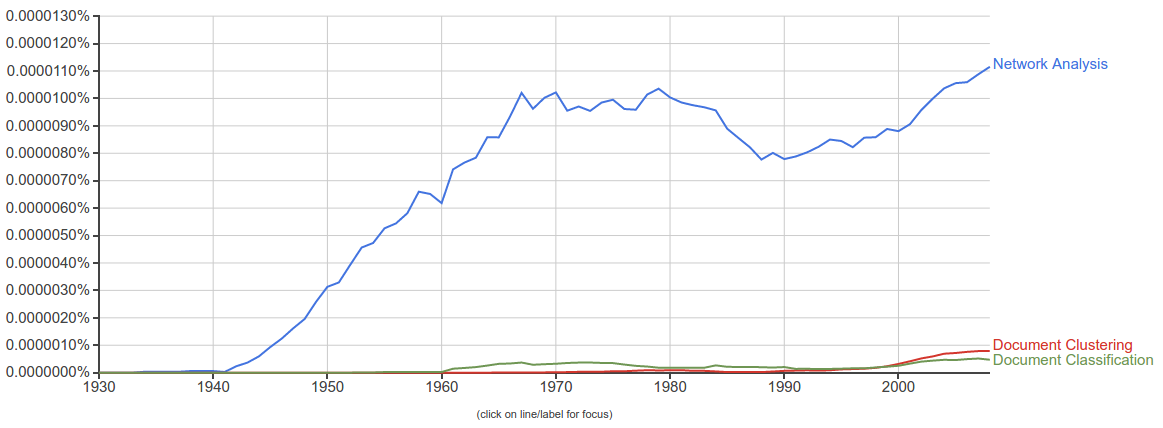
\includegraphics[width=13.7cm]{ngram-viewer/ngram_viewer}}
    \caption[Frequencies of the four research topics discussed found in materials printed between 1930 and 2008 within Google's text corpus.]{Frequencies of the four research topics discussed above found in materials printed between 1930 and 2008 within Google's text corpus. Surprisingly, the search engine was unable to find ngrams for \textit{topic-modelling}.}
    \label{figure:ngram_viewer}
\end{figure}

\iffalse
The Background chapter introduced EPSRC and the problem addressed in this research project while also providing background to several concepts in network science, community detection algorithms and other forms of classification. This section presents the literature reviewed prior to commencing this project identify related works and determine whether studies with a similar focus as this one have already been completed.

\vspace*{1em}

\textbf{Community Structure on Wikipedia} \cite{wikipedia_community_structure} documents community structure thoroughly and provided a good starting point to the literature survey. The article describes the properties and application of community structures in networks. Moreover, it gives a detailed description of a significant number of community detection algorithms as well as several testing methods enabling the evaluation of the algorithms. The information on Wikipedia helped to gain a general understanding of the subject and identify the further direction of the survey.

\vspace*{1em}

\textbf{Community Detection and Mining in Social Media} \cite{community_detection_class} is a class taught by \textit{Lei Tang} (Yahoo! Labs) and \textit{Huan Liu} (Arizona State University) at Arizona State University. The class follows the teachings of a book with the same name \cite{tang2010community} published by \textit{Lei Tang} and \textit{Huan Liu} in 2010. The information from the class is available online in the form of PowerPoint presentations. Essentially, they provide a summary, highlighting the most important parts from the book. The class added the academic knowledge required to the literature survey while also expanding on the information gathered from Wikipedia in regards to community detection evaluation.

\vspace*{1em}

\textbf{Community structure in social and biological networks} \cite{girvan2002community} is a research paper authored by \textit{Michelle Girvan} and \textit{Mark EJ Newman} and published in 2002. The research paper introduces the community structure property, present in many networks. It defines the community structure of a network as network nodes linked together in densely connected clusters, between which there are only sparser connections.

Girvan and Newman also propose a method to detect communities in networks which is built based on the idea of centrality indices. The method is tested on both \textit{real-world} and \textit{computer-generated} networks whose community structure is both known and unknown. \textit{Real-world} networks used for testing include \textit{Zachary's Karate Club Study} and \textit{College Football}. The study used networks without a known community structure such as the \textit{Collaboration} and \textit{Food Web} networks. In the case of a known community structure, the authors found that the method performed well and identified the known community structure with high-sensitivity and reliability. Furthermore, in both cases of unknown community structure, the method still detected significant and informative community divisions.

This research paper was extremely beneficial as it provided further knowledge in the field of community detection as well as the concepts and methods required to complete this research project.

\vspace*{1em}

\textbf{Finding and evaluating community structure in networks}
\cite{newman2004finding} is another paper published in 2004 by \textit{Mark EJ Newman} and \textit{Michelle Girvan} and similar to their previous collaborative work, \textit{Community structure in social and biological networks}. In this publication, the authors propose a set of algorithms for identifying community structure in networks, which is defined as "natural divisions of network nodes into densely connected subgroups." Moreover, this paper represents the introduction of the community structure measure known as \textit{modularity}.

The proposed algorithms include shortest-path betweenness, resistor networks and random walks. A way to measure the strength of the community structure identified by the algorithms proposed is also introduced. The measure provides an objective metric for determining the number of communities a network should be divided into. Testing the algorithms on both \textit{computer-generated} and \textit{real-world networks}, \textit{Newman} and \textit{Girvan} demonstrate that the algorithms are extremely effective at identifying community structure.

The knowledge gained from this study was extremely helpful throughout the duration of this project. It explained how the algorithms proposed were built and how they work, while also providing examples of networks on which the algorithms were evaluated on. It also showed the progress of \textit{Newman} and \textit{Girvan} in the subject since their previous collaborative research effort.

\vspace*{1em}

\textbf{Topic oriented community detection of rating based social networks} is a study conducted by \textit{Reihanian et al.} \cite{reihanian2015topic} in 2015 focusing on community detection from the perspective of content analysis. Most community detection research chooses to focus only on the topological structure of the network. In a social network, for example, this is usually based on the number of communications among individuals. In contrast, this research paper aims to go further and explore and analyse the network's content flow.

The development process of the project commences by preprocessing and annotating topic labels and continues with the clustering of social objects and the creation of topic clusters. It concludes by applying a community detection algorithm to the produced topical clusters in order to identify the community structure within each cluster. Furthermore, a number of experiments are carried out on several data sets including \textit{Movielens 100k}, \textit{Book-Crossing}, \textit{CIAO}, \textit{MovieTweetings} and \textit{Movielens Latest}. It makes use of a performance metric, \textit{purity}, as defined by Zhao et al. \cite{zhao2012topic} which considers both topic and linkage structure. It identifies a maximum \textit{purity} value in each experiment as the topical clusters created in each data set incorporate members which are interested in the same unique topics.

Moreover, the study also compares the topic-oriented community detection proposed with the classical community detection method in which topical content is not analysed. It finds higher values of \textit{modularity} and \textit{purity} in the topic-oriented framework, as the basic network is partitioned into topical clusters, and members who have the same topic of interest are clustered into the same identified community.

\textit{Topic oriented community detection of rating based social networks} has similarities to this project in terms of the focus on topic analysis. It added a new, different perspective to the process of community structure detection which is extremely interesting and definitely a potential path of extending research.

\vspace*{1em}

\textbf{Community detection algorithms: a comparative analysis} is a research paper published by \textit{Lancichinetti et al.} \cite{lancichinetti2009community} in 2009 focusing on the comparison of a wide range of community detection algorithms. Two evaluation benchmarks are employed, the \textit{GN benchmark} by \textit{Girvan} and \textit{Newman} and the \textit{LFR benchmark} proposed by \textit{Lancichinetti et al.}

The community detection algorithms are tested on each evaluation benchmark and include the \textit{Fast greedy modularity optimization}, \textit{Exhaustive modularity optimization via simulated annealing}, \textit{Cfinder},  \textit{Markov Cluster}, \textit{Expectation-maximization} and \textit{Potts model approach}. Furthermore, a number of different graphs were used in the evaluation such as \textit{undirected} and \textit{unweighted} graphs, \textit{directed} and \textit{unweighted} graphs, \textit{undirected} and \textit{weighted} graphs and \textit{undirected} and \textit{unweighted} graphs with overlapping communities. On both evaluation benchmarks, the study found that the \textit{Dynamic algorithm (Infomap)} by \textit{Rosvall} and \textit{Bergstrom} performed the best. The \textit{Fast modularity optimization} by \textit{Blondel et al.} and the \textit{Potts model approach} by \textit{Ronhovde} and \textit{Nussinov} also had a good performance in the evaluation.

This comparative analysis served as a significant source of knowledge in terms of the community detection algorithms available, how they work, when they work best and on which networks. It definitely had an impact on the decisions made in this project in regards to community detection methods utilised. 

\vspace*{1em}

\textbf{On Accuracy of Community Structure Discovery Algorithms} is another comparative study authored by \textit{Orman et al.} \cite{orman2011accuracy} in 2011. It evaluates the majority of algorithms evaluated in \textit{Community detection algorithms: a comparative analysis}, with the exception of \textit{SpinGlass} by \textit{Reichardt} and \textit{Bornholdt} and \textit{Walktrap} by \textit{Pons} and \textit{Latapy}. A generated benchmark graph using the \textit{LFR benchmark} is used. This means that only artificial networks are taken into consideration while the community structure is already known. Each of the eleven community detection algorithms presented are tested on all generated network samples.

The study found that in all cases the \textit{Dynamic algorithm (Infomap)} by \textit{Rosvall} and \textit{Bergstrom} performed better than all other algorithms. \textit{Infomap} succeeded in identifying the communities even for high mixing coefficient values. Furthermore, \textit{Walktrap}, \textit{Markov Cluster}, \textit{Spinglass} and \textit{Louvain} also had an excellent performance level, although not as good as \textit{Infomap}. The research also discovered that for all algorithms, the higher the degree, the better the performance. Moreover, when the network size increases, some algorithms (\textit{Infomap}, \textit{Infomod}, \textit{Louvain}) performed better, others performed worse (\textit{Commfind}, \textit{SpinGlass}, \textit{LeadingEigenvector}, \textit{Radetal}) while the performance of the remaining algorithms (\textit{Walktrap}, \textit{FastGreedy}, \textit{MarkovCluster}) did not change.

This publication served as a reliability test which determined whether the findings in \textit{Community detection algorithms: a comparative analysis} were consistent when compared to other studies. The findings were indeed consistent as both studies identified more or less the same high-performance and low-performance algorithms. This helped to further solidify the decisions taken surrounding community detection algorithms in this thesis project.

\vspace*{1em}

\textbf{Analysis of Citation Networks} is a university project lead by \textit{Anita Valmarska} and \textit{Janez Dem\u{s}ar} at \textit{Jo\v{z}ef Stefan Institute} in \textit{Ljubljana}, \textit{Slovenia}. It focuses on the analysis of citation networks defined as directed networks where one research paper cites another. The data comprises of a collection of 63826 unique psychology-related papers crawled from \textit{Wikipedia} and \textit{Microsoft Academic Research data (MAS)}.

The resulting network consists of 3918 vertices connected by 5732 edges. The study employs the \textit{Louvain} method for the detection of community structure in the created network. The community detection algorithm detected 52 communities with the smallest cluster consisting of 7 research papers, while the largest cluster was constructed of 230 psychology-related publications. The study finds that the results produced have potential as the representation of the communities reveals sensible relationships between psychology sub-fields.

\textit{Analysis of Citation Networks} is the closest in terms of scale to this research project and provides an example of the data, algorithms and tools that other researchers used. Furthermore, it yields new knowledge and inspiration which contributed to the analysis process of this thesis project.
\fi